% Template for PLoS
% Version 3.1 February 2015
%
% To compile to pdf, run:
% latex plos.template
% bibtex plos.template
% latex plos.template
% latex plos.template
% dvipdf plos.template
%
% % % % % % % % % % % % % % % % % % % % % %
%
% -- IMPORTANT NOTE
%
% This template contains comments intended 
% to minimize problems and delays during our production 
% process. Please follow the template instructions
% whenever possible.
%
% % % % % % % % % % % % % % % % % % % % % % % 
%
% Once your paper is accepted for publication, 
% PLEASE REMOVE ALL TRACKED CHANGES in this file and leave only
% the final text of your manuscript.
%
% There are no restrictions on package use within the LaTeX files except that 
% no packages listed in the template may be deleted.
%
% Please do not include colors or graphics in the text.
%
% Please do not create a heading level below \subsection. For 3rd level headings, use \paragraph{}.
%
% % % % % % % % % % % % % % % % % % % % % % %
%
% -- FIGURES AND TABLES
%
% Please include tables/figure captions directly after the paragraph where they are first cited in the text.
%
% DO NOT INCLUDE GRAPHICS IN YOUR MANUSCRIPT
% - Figures should be uploaded separately from your manuscript file. 
% - Figures generated using LaTeX should be extracted and removed from the PDF before submission. 
% - Figures containing multiple panels/subfigures must be combined into one image file before submission.
% For figure citations, please use "Fig." instead of "Figure".
% See http://www.plosone.org/static/figureGuidelines for PLOS figure guidelines.
%
% Tables should be cell-based and may not contain:
% - tabs/spacing/line breaks within cells to alter layout or alignment
% - vertically-merged cells (no tabular environments within tabular environments, do not use \multirow)
% - colors, shading, or graphic objects
% See http://www.plosone.org/static/figureGuidelines#tables for table guidelines.
%
% For tables that exceed the width of the text column, use the adjustwidth
% environment as illustrated in the example table in text below.
%
% % % % % % % % % % % % % % % % % % % % % % % %
%
% -- EQUATIONS, MATH SYMBOLS, SUBSCRIPTS, AND SUPERSCRIPTS
%
% IMPORTANT
% Below are a few tips to help format your equations and other special
% characters according to our specifications. For more tips to help reduce the
% possibility of formatting errors during conversion, please see our LaTeX
% guidelines at http://www.plosone.org/static/latexGuidelines
%
% Please be sure to include all portions of an equation in the math environment.
%
% Do not include text that is not math in the math environment. For example, CO2 will be CO\textsubscript{2}.
%
% Please add line breaks to long display equations when possible in order to fit size of the column. 
%
% For inline equations, please do not include punctuation (commas, etc) within
% the math environment unless this is part of the equation.
%
% % % % % % % % % % % % % % % % % % % % % % % % 
%
% Please contact latex@plos.org with any questions.
%
% % % % % % % % % % % % % % % % % % % % % % % %

\documentclass[10pt,letterpaper]{article}
\usepackage[top=0.85in,left=2.75in,footskip=0.75in]{geometry}

% Use adjustwidth environment to exceed column width (see example table in text)
\usepackage{changepage}

% Use Unicode characters when possible
\usepackage[utf8]{inputenc}

% textcomp package and marvosym package for additional characters
\usepackage{textcomp,marvosym}

% fixltx2e package for \textsubscript
\usepackage{fixltx2e}

% amsmath and amssymb packages, useful for mathematical formulas and symbols
\usepackage{amsmath,amssymb}

% cite package, to clean up citations in the main text. Do not remove.
\usepackage{cite}

% Use nameref to cite supporting information files (see Supporting Information section for more info)
\usepackage{nameref,hyperref}

% line numbers
\usepackage[right]{lineno}

% ligatures disabled
\usepackage{microtype}
\DisableLigatures[f]{encoding = *, family = * }

% rotating package for sideways tables
\usepackage{rotating}

% Remove comment for double spacing
\usepackage{setspace} 
\doublespacing

\usepackage{rotating} % make your own prime symbol
\usepackage{adjustbox} % make your own prime symbol

% Text layout
\raggedright
\setlength{\parindent}{0.5cm}
\textwidth 5.25in 
\textheight 8.75in

% Bold the 'Figure #' in the caption and separate it from the title/caption with a period
% Captions will be left justified
\usepackage[aboveskip=1pt,labelfont=bf,labelsep=period,justification=raggedright,singlelinecheck=off]{caption}

% Use the PLoS provided BiBTeX style
\bibliographystyle{plos2015}

% Remove brackets from numbering in List of References
\makeatletter
\renewcommand{\@biblabel}[1]{\quad#1.}
\makeatother

% Leave date blank
\date{}

% Header and Footer with logo
\usepackage{lastpage,fancyhdr,graphicx}
\usepackage{epstopdf}
\pagestyle{myheadings}
\pagestyle{fancy}
\fancyhf{}
\lhead{\includegraphics[width=2.0in]{/home/jorgsk/Dropbox/The-Tome/my_papers/kinetic_initiation/illustrations/PLOS-submission.eps}}
\rfoot{\thepage/\pageref{LastPage}}
\renewcommand{\footrule}{\hrule height 2pt \vspace{2mm}}
\fancyheadoffset[L]{2.25in}
\fancyfootoffset[L]{2.25in}
\lfoot{\sf PLOS}

%% Include all macros below

\newcommand{\FIG}{{Fig.}}
\newcommand{\FIGS}{{Figs.}}
\newcommand{\SUBSECTION}{\subsection*}

% Your own prime symbol.
\newcommand*{\ppp}{\adjustbox{raise=0.4ex, right=0.56ex}{\scalebox{0.7}{$'$}}\;}

%% END MACROS SECTION

\begin{document}
\vspace*{0.35in}

% Title must be 250 characters or less.
% Please capitalize all terms in the title except conjunctions, prepositions, and articles.
\begin{flushleft}
{\Large
\textbf\newline{The Speed of Transcription Is the Same for Promoter Bound and
Elongating RNA Polymerase}
}
\newline
\\
Jørgen Skancke\textsuperscript{1,*},
Nadav S.\ Bar\textsuperscript{1}
\\
\bigskip
\bf{1} Department of Chemical Engineering, Norwegian University of Science and
Technology, Trondheim, Sør-Trøndelag, Norway
\bigskip

% Use the asterisk to denote corresponding authorship and provide email address in note below.
* jorgsk@nt.ntnu.no

\end{flushleft}
% Please keep the abstract below 300 words
\section*{Abstract}
\parttitle{Background}
During initial transcription, promoter-bound RNA polymerase (RNAP) pulls the
DNA template through the enzyme's active site via the mechanism of scrunching.
This mechanism induces strain on the initial transcribing complex, which may
provoke either an abortive RNA release or promoter escape, two competing
pathways that determine the rate of initiating RNAP that may proceed to
transcription elongation. Despite detailled experimental investigation in the
recent decade, the rate kinetics of these pathways are not entirely clear.

\parttitle{Results} 
We developed a simple model that describes forward transcription and
backtracking of promoter-bound RNAPs. We combined abortive probability data
acquired from bulk experiments with data for the time RNAP spends in abortive
cycles taken from single molecule measurements on the N25 promoter and
identified the rate constants for our model. More specifically, we found the
kinetic rates of backtracking, the nucleotide addition cycle, and unscrunching
and abortive RNA release. Our results show that the average speed of
promoter-bound transcription is similar to the speed attained after promoter
escape.  Additionally, the results suggest that the rate limiting step of
initial transcription is unscrunching and abortive RNA release, consistent
with previous evidence. Moreover, our model predicts that only 4\% of initial
transcription events have a duration less than 1 seconds, in contrast with
previous suggestions (20\%).  

\parttitle{Conclusions}
Taken together, we propose that the strain caused by scrunching does not have
a strong impact on the average speed of transcription by promoter-bound RNAP.


% Please keep the Author Summary between 150 and 200 words
% Use first person.
\section*{Author Summary}
The enzyme RNA polymerase (RNAP) is responsible for reading the genetic code.
It travels along DNA, producing RNA molecules that may in turn be used to make
protein. To begin reading DNA, RNAP must first bind tighly to a promoter
region of DNA. Since it is bound to the promoter, RNAP cannot immediately
travel along DNA when it begins to produce RNA. Instead, when the first part
of RNA is made, DNA must be pulled into RNAP. As more and more DNA is pulled
in, strain builds up. One way this strain can be released is if DNA goes out
again from within the enzyme. If so, the short RNA made becomes released from
RNAP and RNA production must start over. This all happens very fast, which has
made it difficult to measure the speed of the process. In this paper, we have
made a kinetic model for the repeated production and release of short RNAs
from promoter bound RNAPs. By comparing with experimental data, we find that
promoter bound RNAP makes RNA at the same speed as promoter-free RNAP. This
implies that the strain of pulling in DNA does not affect the reaction steps
involved in RNA synthesis.


\linenumbers

\section*{Introduction}
Points:

* Review of kinetic experiments of initial transcription (single molecule and
ensemble; with the limitations of both; sensitivity and time-resolution), as
well kinetic modeling (Xue; did they use michaelise menten rates corresponding
to 1000 $\mu$M?). Mention a word about elongation experiments, of which there
are several.

* Review backtracking, contrasting elongation with initiation.

* Review AP in relation to backtracking, mention GreB. Review the strengths
and weaknesses of AP: when using GreB the probability to backtrack is not
changed, but cleavage happens before abortive product release.

*


\section*{Materials and Methods}
%\addbibresource{/home/jorgsk/Dropbox/phdproject/bibtex/jorgsk.bib}
\SUBSECTION{Kinetic model of initial transcription}
Our model describes the process of initial transcription by considering the
following reactions: i) the NAC ii) backtracking iii) unscrunching and abortive
RNA release (UAR), and iv) promoter escape (\FIG~\ref{fig:model_and_rates}).
We refer to backtracking here only as the first unscrunching step, also known as
backstepping. We find the rate constant of backtracking using APs calculated
from experimental data \cite{hsu_quantitative_1996}. The method relies on two
key points. The first is that the reactions of the NAC and backtracking are in
kinetic competition (\FIG~\ref{fig:model_and_rates}). The second is the
assumption that the probability to backtrack at any given template position is
equal to the AP at that position. In combination, we get
\begin{equation*}
    \frac{b_i}{b_i + \text{NAC}_i} = \text{AP}_i,
\end{equation*}
where subscript $i$ indicates position, and NAC and $b$ are the rate constants
of the nucleotide addition cycle and backtracking, respectively. From this
expression, we obtain an expression for the rate constant for backtracking:
\begin{equation}
  b_i = \frac{\text{NAC}_i\cdot\text{AP}_i}{1-\text{AP}_i}.
  \label{eq:backtrackingcalc}
\end{equation}
\FIG~\ref{fig:param_estimation_scheme} contains an example calculation of rate
constants of backtracking when NAC = 10 $s^{-1}$.

We present a rationale for why APs calculated from abundance of aborted RNA
give a good indication of the probability of the initial backtracking step.
The alternative would be that RNAP could backtrack without
producing an abortive RNA, by entering and remaining in long backtracked
pauses, as has been observed for elongating complexes
\cite{shaevitz_backtracking_2003}. In the data we use for rate constant
estimation, GreB was specifically included in the experiments to avoid long
backtracked pauses, and no such pauses were reported
\cite{revyakin_abortive_2006}. Additionally, it is likely that the shortened
RNA-DNA hybrid and strain from scrunching make backtracked initial
transcribing complexes far less stable than their elongating counterparts. We
therefore find it reasonable to assume that once backtracking has commenced in
initial transcription, an abortive RNA is eventually released. Another
possibility is that abortive RNAs can be released instantly without
backtracking via hyper forward translocation. However, this has only been
described for long abortive transcripts ($>$~16 nt) in N25 promoter mutation
variants \cite{chander_alternate_2007, chander_mechanisms_2015}. Since native
N25's abortive RNAs are shorter than 12 nt \cite{chander_alternate_2007}, we
assume that hyper forward translocation does not take place during initial
transcription on native N25 and that backtracking is the only mechanism
leading to the release of an abortive RNA.

In this work we use both APs obtained for the absence of GreB (-GreB) and in
the presence of GreB (+GreB). When GreB is present, backtracked complexes may
be rescued by GreB stimulated cleavage of the unaligned 3\ppp end of the
transcript. Therefore, APs obtained in the presence of GreB represent the
combined probability of both backtracking and avoiding rescue by GreB until
RNA is released. We therefore assume that when GreB is present, GreB-mediated
cleavage and subsequent NACs are rapid steps compared to unscrunching; this is
supported by the finding that unscrunching and abortive RNA release are slow
relative to NAC \cite{revyakin_abortive_2006, margeat_direct_2006}. This
permits using the APs obtained in the presence of GreB as effective
backtracking probabilities. The +GreB AP values used in this work are obtained
from Figure 4B in Hsu et al. \cite{hsu_initial_2006}, and -GreB AP values have
been calculated directly from raw data used to build Table 1 in Hsu et al.\
\cite{hsu_initial_2006} (data provided by Lilian M. Hsu). AP values in Hsu et
al.\ have been obtained in the presence of $100\ \mu M$ NTP at 37 $^{\circ}$C
\cite{hsu_initial_2006}.

\SUBSECTION{Implementation and rate constant estimation}
A central result in this work is the estimation of the rate constants of initial
transcription. We perform this estimation by running multiple simulations with
different combinations of rate constants and evaluating the fitness of each
combination to experimental data. The data used for rate constant estimation
is the distribution of time spent in abortive cycling on the N25 promoter
determined by Revyakin et al.\ \cite{revyakin_abortive_2006}. This data was
obtained under $100\ \mu M$ NTP at 34 $^{\circ}$C, near-identical conditions
to how the APs were obtained \cite{hsu_initial_2006}.

The experimental data was obtained from 100 individual initial transcription
events \cite{revyakin_abortive_2006}. For experiments with single molecules,
there is an inherent stochastic component in the experimental outcome that
derives from the randomness of molecular motion. That this is evident for
transcription can be inferred from the large variation in the speed of
transcription elongation observed in single-molecule experiments
\cite{adelman_single_2002, tolic-norrelykke_diversity_2004}. To account for
this randomness, we perform the kinetic simulations using the Gillespie
algorithm for stochastic simulations of chemical reactions
\cite{gillespie_exact_1977}. Specifically, we make use the version implemented
by Maarleveld et al.\ in the StocPY software \cite{maarleveld_stochpy:_2013}.

The procedure for rate constant estimation (illustrated in
\FIG~\ref{fig:param_estimation_scheme}) is as follows (rate constant names
are given in \FIG~\ref{fig:model_and_rates}): First, we assign random values
to the three rate constants NAC ($k_n$), promoter escape ($k_e$) and
unscrunching and abortive RNA release ($k_u$) within certain fixed boundaries
(see below). These values are chosen independently from a uniform
distribution. Second, we use the rate constant of the NAC and APs to
calculate the rate constant of backtracking ($k_b$) using
Eq.~(\ref{eq:backtrackingcalc}). We then simulate 100 initial transcription
events and calculate the distribution of time spent in abortive cycling as a
result of these specific rate constants. The result is measured against the
empirical distribution \cite{revyakin_abortive_2006} using the root mean
square error. By repeating this procedure several times, we obtain statistics
of which values of rate constants are associated with the best match with
the experimental data. By virtue of using stochastic simulations, one does not
arrive at a unique set of rate constants that have optimal fit with data; if a
simulation is repeated with identical rate constants, slightly different
results will be obtained due to the inherent stochasticity of the reaction
process. Therefore, we identify the best-fitting rate constants from peak of
the fitness distribution, i.e.\ identify those rate constants that stand out
by most often giving the best fit to data.

The boundaries of the rate constants for parameter estimation were chosen from
extrema estimated from experimental findings. The speed of the NAC during initial
transcription cannot be much less than 3 nt/s, since Revyakin et al.\ measured
2.5 seconds as the shortest duration of abortive cycling
\cite{revyakin_abortive_2006} to cover the $\sim 11$ nts required for promoter
escape on N25. At the same time, it should not be larger than 25 nt/s,
which is above the upper limit of what has been measured for transcription
elongation \cite{bai_mechanochemical_2007}. While it is not clear how
transcription would proceed faster for promoter-bound RNAP, we use 25 nt/s as
a maximum value also in order to see if the model is able to discard these
extreme values during rate constant estimation. For backtracking and abortive
RNA release, it is known that the rate constant must be faster than 1
s$^{-1}$, since this was the time-resolution of experimental equipment which
could not resolve this value \cite{revyakin_abortive_2006}. To explore
possible values for all rate constants equally, we set the minimum and maximum
values of all rate constants to be 1 s$^{-1}$ and 25 s$^{-1}$, respectively. 

\begin{figure}[h]
    \begin{center}
      
\includegraphics{../illustrations/model_and_rates_mini}
    \end{center}
  \caption{{\bf Kinetic model of initial transcription on the N25 promoter.}
    From the open complex (OC) transcription proceeds by NACs from one initial
    transcribing complex (ITC) to the next, where each ITC is identified in
    subscript by the length of its nascent RNA. Initial transcription proceeds
    until the nascent RNA has reached the experimentally obtained maximum size
    of abortive transcript; for N25, this is 11 nt \cite{hsu_initial_2006}.
    For ITCs with an RNA of 2 nt in length or longer, there is a competition
    between the NAC and backtracking. Backtracking causes termination of
    transcription, and only further backtracking (unscrunching) and abortive
    RNA release may follow, returning RNAP to the open complex. From the open
    complex, forward transcription may resume once more. The names of the rate
    constants are as follows: $k_n$ (NAC), $k_e$ (promoter escape), $k_u$
    (unscrunching and abortive RNA release) and $k_{b,i}$ (backtracking).}
    \label{fig:model_and_rates}
\end{figure}

\begin{figure}[h]
    \begin{center}
      \includegraphics{../illustrations/parameter_estimation_scheme}
    \end{center}
  \caption{ {\bf Rate constant estimation protocol.} \textbf{1:}
    Rate constants for the NAC, UAR and promoter escape are randomly sampled
    from a uniform distribution (example values are shown). Of these values,
    the NAC is used further to obtain backtracking rates at each template
    position (\textbf{3}). This is done by solving
    Eq.~(\ref{eq:backtrackingcalc}), where the APs are obtained from Hsu et
    al.\ \cite{hsu_initial_2006} (\textbf{2}). The backtracking rate
    constants, together with the NAC, UAR, and promoter escape rate constants
    sampled in step \textbf{1}, encompass the complete kinetic scheme of
    initial transcription (\textbf{4}). This scheme is then used to simulate
    the kinetics of 100 initial transcription events; from these 100 events
    the distribution of time spent in abortive cycling is calculated and
    compared to measured data from Revyakin et al.\
    \cite{revyakin_abortive_2006} (\textbf{5}). From the distance between the
    measured distribution and the simulated distribution, a fitness score is
    produced. This score is associated to the three randomly selected rate
    constants in step \textbf{1}, and is a measure for how well the kinetic
    scheme (the three random rate constants and the AP values) agree with the
    experimental data. By repeating steps \textbf{1}-\textbf{5} multiple
    times, distributions are obtained from where we find which values of the
    rate constants provide the best fit with experimental data.}
    \label{fig:param_estimation_scheme}
\end{figure}


% Results and Discussion can be combined.
\section*{Results}
%\addbibresource{/home/jorgsk/Dropbox/phdproject/bibtex/jorgsk.bib}
\subsection{The forward pathway of transcription proceeds at the same rate
for initial transcription as for elongation}
Revyakin et.\ al measured initial transcription on the N25 promoter in the
presence of GreB and 100 $\mu$M NTP and found that abortive cycling lasts on
average 5 seconds prior to promoter escape~\cite{revyakin_abortive_2006}. We
constructed a kinetic model of initial transcription and fitted it to this
distribution, leveraging the APs quantified from +GreB experiments of initial
transcription by Hsu et. al~\cite{hsu_initial_2006}
(Figure~\ref{fig:revyakin_fit}). The rate constants that resulted in 
optimal fit with data were as follows:~NAC 10.5 s$^{-1} \pm 0.64$; escape
11.84 s$^{-1} \pm 1.81$; and unscrunching 1.58 s$^{-1} \pm 0.14$ (Figure
\ref{fig:parameter_estimation}, Table~\ref{tab:param_fit_revyakin}). The value
for NAC before promoter escape is highly similar to transcription velocity
after promoter escape: 9.5 nt s$^{-1}$ for positively supercoiled DNA and 13.8
nt s$^{-1}$ for negatively supercoiled DNA~\cite{revyakin_abortive_2006}. This
indicates that NAC proceeds at the same rate for both scrunching and
transcription elongation. The comparatively lower rate of 1.58 s$^{-1}$ for
unscrunching and abortive RNA release is consistent with previous reports that
this process is rate limiting for initial
transcription~\cite{margeat_direct_2006, revyakin_abortive_2006}. Revyakin
et.\ al did not measure rounds of abortive cycling that lasted shorter than 1
second, but proposed based on extrapolation of their data that 20\% of
abortive cycles last shorter than one second \cite{revyakin_abortive_2006}.
The best fit to the data by our kinetic model suggests that less than 2\% of
abortive cycling rounds last shorter than 1 second (Figure
\ref{fig:revyakin_fit}). This number can be understood by considering that
with a transcription rate of $10.5$~nt s$^{-1}$ it takes around one second to
reach promoter escape on N25 if backtracking is avoided. Indeed, when fitting
the model to the extrapolation of the Revyakin et. al data, a rate constant
for the NAC of 18.4 s$^{-1} \pm 3.8$ was obtained
(Table~\ref{tab:param_fit_revyakin}), which is higher than what is reported
for transcription elongation for the same experiment
\cite{revyakin_abortive_2006}.

\begin{figure}
	\begin{center}
      \includegraphics[scale=0.8]{../illustrations/estimated_parameters.pdf}
	\end{center}
    \caption{Estimation rate constants for +GreB N25. (NOTE: values are just
    placeholders for now)}
    \label{fig:parameter_estimation}
\end{figure}

\subsection{Estimated rate constants are also valid for -GreB kinetics}
We estimated the rate constants of NAC, escape, and backtracking and abortive
RNA release using APs associated with +GreB. However, once fitted, the rate
constants should be generally valid. The fitted model should therefore be able
to capture the kinetics of transcription on N25 for different APs, such as the
one obtained for transcription under -GreB conditions, for which the abortive
probability is considerably higher \cite{hsu_initial_2006}. To test this, we
used the estimated rate constants to simulate initial transcription for -GreB
conditions. We compared the simulation result with the kinetics of FL
transcript synthesis reported by Vo et.\ al \cite{vo_vitro_2003-1}. The
half-life of FL transcript synthesis, denoted $\tau$, was 15.5 s in the
simulation, and determined to be 13.7 s in the experiment after fitting
measurements to a single exponential (Figure~\ref{fig:vo_comparison}). While these
numbers appear close, there is no other kinetic data for the N25 promoter in
the literature which can tell us the range of values of $\tau$ for initial
transcription on N25. To therefore be able to say something about the
variability of $\tau$, calculated this value from simulations of initial
transcription on N25-anti and N25 A1-anti, two ITS variants of N25 which have
previously been shown to vary compared to N25 in several quantitative
parameters for initial transcription~
\cite{hsu_initial_2006,chan_anti-initial_2001,kammerer_functional_1986}. This
resulted in values of $\tau$ of 61.2 s for N25-anti and 179.6 s for N25
A1-anti, which agrees with these ITS variants having a lower productive yield
than N25 \cite{hsu_initial_2006}. This shows that the experimentally obtained
and simulated values for $\tau$ for N25 -GreB are similar relative to values
(Figure \ref{fig:its_variant_fl_comparison}).

\subsection{Estimated rate constants are sensitive to changes to the +GreB 
APs}
In estimating the rate constants, we have used APs from bulk studies by Hsu
et. al \cite{hsu_initial_2006} together with an abortive cycling distribution
obtained from single-molecule studies by Revyakin et. al
\cite{revyakin_abortive_2006}. This relies on the assumption that the
position-specific probability to abort initial transcription is the same for
the single-molecule experiment as as for the bulk studies. That this holds
true is not known, since the rapid kinetics of initial transcription
has prevented direct observation of the exact position of backtracking and abortive
RNA release \cite{margeat_direct_2006, revyakin_abortive_2006}. One way to
assess the similarity of the two abortive profiles is to quantify the
sensitivity of the estimated rate constants to changes in the APs. We would
argue that the rate constants in Table~\ref{tab:param_fit_revyakin},
specifically the NAC and backtracking and abortive RNA release, are consistent
available literature; therefore, if we can find a dose-response tendency
where modifying the AP values from their +GreB baseline leads to
unphysiological rate constants or otherwise worsened model performance, this
is an indication that the original bulk AP values are also descriptive for the
single-molecule experiment. The first kind of perturbation we tested was to
replace the +GreB APs with -GreB APs, and then repeat the estimation
procedure. This led to an estimate for the rate constant of NAC of 20.9
s$^{-1} \pm 2.9$ (Table~\ref{tab:param_fit_revyakin}). We consider this value
unphysiological since it would suggest that NAC proceeds nearly twice as fast during
scrunching compared to elongation, proceeding at speeds normally found for NTP
concentrations of 1000 $\mu$M~\cite{bai_mechanochemical_2007}, 10 times higher
than actual experimental conditions. Next, we performed a more general
perturbation of the AP values, making them both higher and lower across the
ITS (Figure~\ref{fig:aps_after_adjustment}). This showed first of all that the fit is
best for zero or small perturbations, and gets progressively worse as
perturbations increase (Figure \ref{fig:ap_adjustment}A), which shows that the
original bulk +GreB AP values lie in an optimal region in terms of fitting the
the single-molecule experimental data. The effect of perturbations on the rate
constants were as follows: for higher AP, NAC is forced to increase to
maintain optimal fit, while NAC decreases when AP is lowered, (Figure
\ref{fig:ap_adjustment}B); the rate constant for unscrunching
and abortive release similarly increased as AP increases, to the point where
this step becomes nearly as rapid as the NAC, but for lower AP this value was
not much removed from the baseline (Figure \ref{fig:ap_adjustment}C). The rate
constant for promoter escape was insensitive to changes in AP, indicating that
model performance is insensitive to this parameter (Figure
\ref{fig:ap_adjustment}D). We therefore observed that for an increased AP, the
rate constant for NAC increased to the point of being unphysiological at more
than 20 $s^{-1}$, and the rate constant for the abortive step increased to the
point of being similar in size to that of the NAC, where it is hardly rate
limiting for the process. However, for a reduced AP there is no published data
by which to judge the rate constants as unphysiological. Therefore, we wished
to assess how the rate constants optimal for low APs would affect model
performance. To do so, we used these rate constants to obtain $\tau$ for -GreB
APs, and calculated the size of this value relative to the one obtained from
measurements from Vo et. al \cite{vo_vitro_2003-1}, where we denote the
relative value as $\tau_r$. This showed that when AP is reduced compared to the
original +GreB values, $\tau$ becomes increasingly large comparing to 
experimental value (Figure \ref{fig:ap_adjustment}E), showing that model
performance worsens when AP is lower than the baseline +GreB values.

\begin{table}
  \label{tab:param_fit_revyakin}
  \caption{Fitted rate constants of initial transcription}
  \begin{center}
    \begin{tabular}{lccc}
       \toprule
       & NAC & Escape & Abort \\
       +GreB & $10.1 \pm 0.6$ & $14.6 \pm 1.8$ & $1.6 \pm 0.1$ \\
       -GreB & $20.9 \pm 2.1$ & $15.3 \pm 5.3$ & $17.5 \pm 5.4$ \\
       Extrapolated fit & $18.4 \pm 3.8$ & $16.6 \pm 6.9$ & $1.8 \pm 1.1$ \\
    \end{tabular}
  \end{center}
\end{table}

\begin{figure}
    \begin{center}
      \includegraphics[scale=0.7]{../figures/cumul_scrunch_fit.pdf}
    \end{center}
    \caption{Initial transcription model fitted to distribution of time spent
      in rounds of abortive cycling before promoter escape. Measurements are
      from Revyakin et.\ al \cite{revyakin_abortive_2006}. Fit to measurements
      shows best fit by an exponential function. The green area indicates time
      is less than one second.}
\label{fig:revyakin_fit}
\end{figure}


\begin{figure}
    \begin{center}
      \includegraphics[scale=0.8]{../figures/ap_adjustment.pdf}
    \end{center}
    \caption{Effect on model fit, estimated rate constants, and model
      performance when AP values are modified from baseline. A) Effect on
      model fit; B) effect on rate constant of NAC; C) effect on rate constant of
      the abortive step; D) effect on rate constant of escape; E) effect on
      $\tau_r$, which is the model-obtained $\tau$ relative to the value found from
      measurements from Vo et.\ al \cite{vo_vitro_2003-1} (Figure
      \ref{fig:vo_comparison}).}
\label{fig:ap_adjustment}
\end{figure}


\begin{figure}
    \begin{center}
        \includegraphics[scale=0.7]{../figures/vo_greb_minus_comparison.pdf}
    \end{center}
    \caption{Kinetics of FL transcript synthesis under -GreB conditions.
      Commparison between model (light green line) and measurements from Vo
      et.\ al \cite{vo_vitro_2003-1} (green dots). Blue line shows fit of
      measurements to a single exponential function.}
\label{fig:vo_comparison}
\end{figure}


\begin{figure}
    \begin{center}
      \includegraphics[scale=0.7]{../figures/Time_to_reach_fifty_percent_of_FL.pdf}
    \end{center}
    \caption{The value of $\tau$ obtained from simulation on -GreB N25 is
      similar to the experimentally obtained value, and is distinct from
      values of $\tau$ obtained by simulation on -GreB ITS variants of N25.}
\label{fig:its_variant_fl_comparison}
\end{figure}

% If you end up short with things in the results section, add something here
% about the sensitivity of the parameters. Define sensitivity as how much the
% value can be varied +/- before a 5% change in best fit is reached?

% Can we say that because the NAC is similar to elongation NAC, and that the
% ensemble experiment was so closely matched, that our two main assumptions
% are justified:
    % 1) that each backtracking event leads to an abortive release?
    % 2) that -GreBassisted cleavage and RNA release is rapid enough to be
    % negligeble for the oveall kinetics of the system?

%But how do we interpret the AP for the +GreB experiments? This is a bit of a
%conundrum. We are interpreting them as if GreB results in a reduction of
%the probability of backtracking at each position. That is OK, though, because
%then we only count the unscrunching steps that have proceeded without
%influence by GreB. We thus assume that rescue upon backtracking is fast
%enough.


\section*{Discussion}
%\addbibresource{/home/jorgsk/Dropbox/phdproject/bibtex/jorgsk.bib}
In this paper we have built a model of initial transcription and fitted rate
constants of key processes using a combination of bulk and single-molecule
experimental data. This allowed us to pin down the essential rate constants of
the process, showing that the speed of transcription highly similar for
initial transcription and transcription elongation
(Figure~\ref{fig:revyakin_fit}, Table~\ref{tab:param_fit_revyakin}). We
validated the rate constants by comparing with published kinetic data of
initial transcription obtained under experimental conditions different than
for how the rate constants were obtained (Figure~\ref{fig:vo_comparison}), and
we showed that the underlying assumption of a common abortive profile between
single-molecule and bulk experiments is likely correct, as departure from this
profile led to unphysiological rate constants and worsening of model
performance (Figure~\ref{fig:ap_adjustment}).

The model of initial transcription used in this work uses the same rate
constant for NAC and unscrunching and abortive release at each template
position (Figure~\ref{fig:model_and_rates}). Therefore, the rate constants
presented here must be considered average values. Given the complex nature of
initial transcription, one may ask if the use of average rate constants is a reasonable
assumption. For T7 RNAP, a kinetic study showed a 10-fold variation for the
NAC rate constant, from 6 nt$^{-s}$ to \cite{tang_real-time_2009}. We would
argue that this is not the case for bacterial RNAP. The average rate constant
we found for NAC matched closely the average speed of transcription during
elongation. Since it is unlikely that the NAC is faster for some steps during
initiation, the closely matching averages require that the NAC cannot be much
slower either. Our results therefore support at model where there is no
bottleneck step during for the NAC during initial transcription, but that
transcription during initiation is the same as for elongation, except that
there is a higher probability to backtrack. This implies that the strain of
the growing DNA bubble and the steric clashes with $\sigma$ do not greatly
affect the NAC during initiation. On the other hand, it is likely that these
processes contribute to the increased rate of backtracking during initiation
compared to those found for elongation.

% XXX new section:
% Add something about the value of NAC, talk about the distribution (it's
% quite wide). Mention the issue of supercoiling, and the case of linear
% fragments. Talk about distributions in general: Abortive and backtracking
% has a very narrow distribution around 1-2, while NAC is more wide, but with
% a clear peak for the highest values around 11.4 whatev. Limitation in
% resolving this resolution is partially in the low number of single
% nucleotide experiments, 100, for which there is plenty of variation in the
% speed of NAC, at lest for elongation.

Our model assumes that APs calculated from the abundance of aborted RNA are
equal to the probability of the initial backstep
(Figure~\ref{fig:model_and_rates}). The alternative would be that some
complexes, especially in the absence of GreB, remain in long backtracked
pauses, as has been observed for transcription elongation
\cite{shaevitz_backtracking_2003}. If long backtracked pauses were common
during initiation, the APs would only reflect those backtracked
complexes that abort, so that that the actual probability to backtrack would
be higher than what is indicated by the APs. However, we showed that rate
constants obtained by fitting a model to +GreB APs are descriptive for the
kinetics of initial transcription without GreB
(Figure~\ref{fig:vo_comparison}), where such long backtracked pauses may take
place. This result indicates that such long backtracked pauses, if they exist,
do not make a large contribution to the kinetics of initial transcription.

The rate constant for unscrunching and abortive RNA release was found to have
a narrow optimum at 1.7 $\pm 0.4$. We speculate that this value may vary for
different template positions. Presumably, backtracking happens more readily
and abortive release is more rapid for an incomplete RNA-DNA hybrid
\cite{nudler_rnadna_1997,komissarova_shortening_2002}. This would imply that
this step is slower for complexes that have obtained with a full-length
RNA-DNA hybrid. For N25, this may not be so relevant, since promoter escape
happens at +11, shortly after a full hybrid has been obtained. To resolve
this number more precisely, experimental techniques are needed that can
resolve backtracking and abortive RNA release at the time scale in which they
occur. Alternatively, as increasingly complex molecular simulations of RNAP
dynamics are obtained \cite{silva_millisecond_2014}, the details of this
process may be instead first be obtained using numerical methods alone.

In conclusion, this work supports a model of initial transcription where the
forward rate of transcription is highly similar to the rate for transcription
elongation, and where the backtracking and abortive release step is more than
5 times slower. Since model fitting resulted in physiologically reasonable
rate constants (Table~\ref{tab:param_fit_revyakin}), and since these rate
constants hold up to independent kinetic data
(Figure~\ref{fig:vo_comparison}), this supports that the assumptions
underlying the model are sound. Therefore, it is likely that the APs
reflect probabilities to backtrack during initial transcription, and it is
probable that the APs are the same for the single-molecule experiments of
Revyakin et.\ al \cite{revyakin_abortive_2006} and the steady state
transcription experiments by Hsu et.\ al \cite{hsu_initial_2006}.
 
% Q:You mentioned something to Itziar, something that you decided not to
% include! Yes, separating the productive from the unproductive transcripts.
% You can do this by analyzing the kinetics from a single round of
% transcription.


%\section*{Supporting Information}

% Include only the SI item label in the subsection heading. Use the
% \nameref{label} command to cite SI items in the text.
%\subsection*{S1 Fig}
%\label{S1_Fig}

\section*{Acknowledgments}
We thank Lilian M. Hsu for thoughtful comments on the manuscript during the
writing process and for sharing experimental data.

\nolinenumbers

%\section*{References}
% Either type in your references using
% \begin{thebibliography}{}
% \bibitem{}
% Text
% \end{thebibliography}
%
% OR
%
% Compile your BiBTeX database using our plos2015.bst
% style file and paste the contents of your .bbl file
% here.
% 

%\bibliography{/home/jorgsk/Dropbox/phdproject/bibtex/jorgsk}
\bibliography{/home/jorgsk/Dropbox/phdproject/bibtex/jorgsk_abr_nodot.bib}
%\begin{thebibliography}{10}

%\bibitem{bib1}
%Devaraju P, Gulati R, Antony PT, Mithun CB, Negi VS. Susceptibility to SLE in South Indian Tamils may be influenced by genetic selection pressure on TLR2 and TLR9 genes. Mol Immunol. 2014 Nov 22. pii: S0161-5890(14)00313-7. doi: 10.1016/j.molimm.2014.11.005

%\bibitem{bib2}
%Huynen MMTE, Martens P, Hilderlink HBM. The health impacts of globalisation: a conceptual framework. Global Health. 2005;1: 14. Available: http://www.globalizationandhealth.com/content/1/1/14.

%\end{thebibliography}


\end{document}
